%%%%%%%%%%%%%%%%%%%%%%%%%%%%%%%%%%%%%%%%%
% Beamer Presentation
% LaTeX Template
% Version 1.0 (10/11/12)
%
% This template has been downloaded from:
% http://www.LaTeXTemplates.com
%
% License:
% CC BY-NC-SA 3.0 (http://creativecommons.org/licenses/by-nc-sa/3.0/)
%
%%%%%%%%%%%%%%%%%%%%%%%%%%%%%%%%%%%%%%%%%

%----------------------------------------------------------------------------------------
%	PACKAGES AND THEMES
%----------------------------------------------------------------------------------------

\documentclass{beamer}

\mode<presentation> {

% The Beamer class comes with a number of default slide themes
% which change the colors and layouts of slides. Below this is a list
% of all the themes, uncomment each in turn to see what they look like.

%\usetheme{default}
%\usetheme{AnnArbor}
%\usetheme{Antibes}
%\usetheme{Bergen}
\usetheme{Berkeley}
%\usetheme{Berlin}
%\usetheme{Boadilla}
%\usetheme{CambridgeUS}
%\usetheme{Copenhagen}
%\usetheme{Darmstadt}
%\usetheme{Dresden}
%\usetheme{Frankfurt}
%\usetheme{Goettingen}
%\usetheme{Hannover}
%\usetheme{Ilmenau}
%\usetheme{JuanLesPins}
%\usetheme{Luebeck}
%\usetheme{Madrid}
%\usetheme{Malmoe}
%\usetheme{Marburg}
%\usetheme{Montpellier}
%\usetheme{PaloAlto}
%\usetheme{Pittsburgh}
%\usetheme{Rochester}
%\usetheme{Singapore}
%\usetheme{Szeged}
%\usetheme{Warsaw}

% As well as themes, the Beamer class has a number of color themes
% for any slide theme. Uncomment each of these in turn to see how it
% changes the colors of your current slide theme.

%\usecolortheme{albatross}
%\usecolortheme{beaver}
%\usecolortheme{beetle}
%\usecolortheme{crane}
%\usecolortheme{dolphin}
%\usecolortheme{dove}
%\usecolortheme{fly}
%\usecolortheme{lily}
%\usecolortheme{orchid}
%\usecolortheme{rose}
%\usecolortheme{seagull}
%\usecolortheme{seahorse}
%\usecolortheme{whale}
%\usecolortheme{wolverine}

%\setbeamertemplate{footline} % To remove the footer line in all slides uncomment this line
%\setbeamertemplate{footline}[page number] % To replace the footer line in all slides with a simple slide count uncomment this line

%\setbeamertemplate{navigation symbols}{} % To remove the navigation symbols from the bottom of all slides uncomment this line
}

\usepackage{graphicx} % Allows including images
\usepackage{booktabs} % Allows the use of \toprule, \midrule and \bottomrule in tables
\usepackage{amsmath}
%----------------------------------------------------------------------------------------
%	TITLE PAGE
%----------------------------------------------------------------------------------------

\title[Kalman Filter for SVO Scale Estimation]{Kalman Filter for SVO Scale Estimation} % The short title appears at the bottom of every slide, the full title is only on the title page

\author{Group D} % Your name
\institute[TUT] % Your institution as it will appear on the bottom of every slide, may be shorthand to save space
{
Tampere University of Technology \\ % Your institution for the title page
\medskip
\textit{joonas.melin@tut.fi} % Your email address
}
\date{\today} % Date, can be changed to a custom date

\begin{document}

\begin{frame}
\titlepage % Print the title page as the first slide
\end{frame}

\begin{frame}
\frametitle{Overview} % Table of contents slide, comment this block out to remove it
\tableofcontents % Throughout your presentation, if you choose to use \section{} and \subsection{} commands, these will automatically be printed on this slide as an overview of your presentation
\end{frame}

%----------------------------------------------------------------------------------------
%	PRESENTATION SLIDES
%----------------------------------------------------------------------------------------

%------------------------------------------------
\section{Motivation} % Sections can be created in order to organize your presentation into discrete blocks, all sections and subsections are automatically printed in the table of contents as an overview of the talk
%------------------------------------------------


\begin{frame}
\frametitle{Motivation}
\begin{itemize}
 \item SVO is performing adequately on the copter with small tuning and minor fixes
 \item The scale and orientation of the visual odometry is still unknown
 \item Kalman Filter can be applied to estimate scale and orientation, how ever, pose of the copter needs to be estimated first
\end{itemize}

\end{frame}

\section{Implementation}
\begin{frame}
 \frametitle{Premises}
 \begin{itemize}
 \item Normal EKF equations for the update, we will list the models used
 \item State $S = \begin{bmatrix}Q_{copter}^{1x4} & P_{position}^{1x3} & V_{velocity}^{1x3} & s_{svo} & Q_{svo}^{1x4}\end{bmatrix}^T$
 \item $Q = \begin{bmatrix}q_w & q_x & q_y & q_z\end{bmatrix}$
 \item $P = \begin{bmatrix}x & y & z\end{bmatrix}$
 \item $V = \begin{bmatrix}x & y & z\end{bmatrix}$
 \end{itemize}
 
\end{frame}


\subsection{Prediction}
\begin{frame}
\frametitle{Prediction}
  \begin{itemize}
    \item $S^{t+1} = FS^{t} + G$
    \item $F = \begin{bmatrix}
  1& 0& 0& 0& 0& 0& 0&  0&  0&  0\\
  0& 1& 0& 0& 0& 0& 0&  0&  0&  0\\
  0& 0& 1& 0& 0& 0& 0&  0&  0&  0\\
  0& 0& 0& 1& 0& 0& 0&  0&  0&  0\\
  0& 0& 0& 0& 1& 0& 0& \Delta t&  0&  0\\
  0& 0& 0& 0& 0& 1& 0&  0& \Delta t&  0\\
  0& 0& 0& 0& 0& 0& 1&  0&  0& \Delta t\\
  0& 0& 0& 0& 0& 0& 0&  1&  0&  0\\
  0& 0& 0& 0& 0& 0& 0&  0&  1&  0\\
  0& 0& 0& 0& 0& 0& 0&  0&  0&  1 
  \end{bmatrix}$
  \end{itemize} 
\end{frame}

\begin{frame}
  \begin{itemize}
  \item $G = \Delta tBU$
  \item $U = \begin{bmatrix}\Delta\alpha_{euler}^{1x3} & A_{acceleration}^{1x3} & g_{gravitation}\end{bmatrix}$
  \item \resizebox{.9\hsize}{!}{$B = \begin{bmatrix}
  -q_x/2& -q_y/2& -q_z/2&                         0&                         0&                         0&  0\\
  q_w/2& -q_z/2&  q_y/2&                         0&                         0&                         0&  0\\
  q_z/2&  q_w/2& -q_x/2&                         0&                         0&                         0&  0\\
 -q_y/2&  q_x/2&  q_w/2&                         0&                         0&                         0&  0\\
     0&     0&     0&                         0&                         0&                         0&  0\\
     0&     0&     0&                         0&                         0&                         0&  0\\
     0&     0&     0&                         0&                         0&                         0&  0\\
     0&     0&     0& q_w^2 + q_x^2 - q_y^2 - q_z^2&         2*q_x*q_y - 2*q_w*q_z&         2*q_w*q_y + 2*q_x*q_z&  0\\
     0&     0&     0&         2*q_w*q_z + 2*q_x*q_y& q_w^2 - q_x^2 + q_y^2 - q_z^2&         2*q_y*q_z - 2*q_w*q_x&  0\\
     0&     0&     0&         2*q_x*q_z - 2*q_w*q_y&         2*q_w*q_x + 2*q_y*q_z& q_w^2 - q_x^2 - q_y^2 + q_z^2& -1
  \end{bmatrix}$} 
  \end{itemize} 
\end{frame}



\subsection{Acceleration update}
\begin{frame}
\frametitle{Acceleration update}
  \begin{itemize}
  \item Measurement is the accelerations measured by the IMU
  \item Measurement model $A_{imu} = R(Q_{copter})A_{gravitation}^{3x1}$
  \item $R$ is an quaternion rotation matrix derived from the state
  \item Jacobian $J = \frac{\partial A_{imu}}{\partial \begin{bmatrix}Q_{copter}^{1x4} & P_{position}^{1x3} & V_{velocity}^{1x3}\end{bmatrix}}$
  \end{itemize} 
\end{frame}

\subsection{GPS update}
\begin{frame}
\frametitle{GPS update}
  \begin{itemize}
  \item Measurement is the position measured by the GPS
  \item Measurement model $P_{gps} = P_{position}$
  \item Jacobian $J = \frac{\partial P_{gps}}{\partial \begin{bmatrix}Q_{copter}^{1x4} & P_{position}^{1x3} & V_{velocity}^{1x3}\end{bmatrix}}$
  \end{itemize} 
\end{frame}

\subsection{Velocity update}
\begin{frame}
\frametitle{Velocity update}
  \begin{itemize}
  \item Measurement is the speed derived from the GPS
  \item Measurement model $V_{gps} = V_{velocity}$
  \item Jacobian $J = \frac{\partial P_{gps}}{\partial \begin{bmatrix}Q_{copter}^{1x4} & P_{position}^{1x3} & V_{velocity}^{1x3}\end{bmatrix}}$
  \end{itemize} 
\end{frame}

\subsection{SVO scale update}
\begin{frame}
\frametitle{SVO scale update}
  \begin{itemize}
  \item Measurement is the velocity measured by the SVO
  \item Measurement model $V_{svo} = R(Q_{svo})(V_{velocity}/s_{svo})$
  \item Jacobian $J = \frac{\partial V_{svo}}{\partial \begin{bmatrix}Q_{copter}^{1x4} & P_{position}^{1x3} & V_{velocity}^{1x3}& s_{svo} & Q_{svo}^{1x4}\end{bmatrix}}$
  \end{itemize} 
\end{frame}

\subsection{SVO orientation update}
\begin{frame}
\frametitle{SVO orientation update}
  \begin{itemize}
  \item Measurement is the orientation quaternion measured by the SVO
  \item Measurement model $Q_{measured} = Q_{svo}Q_{copter}$
  \item Jacobian $J = \frac{\partial Q_{measured}}{\partial \begin{bmatrix}Q_{copter}^{1x4} & P_{position}^{1x3} & V_{velocity}^{1x3}& s_{svo} & Q_{svo}^{1x4}\end{bmatrix}}$
  \end{itemize} 
\end{frame}

\subsection{How it looks like}
\begin{frame}
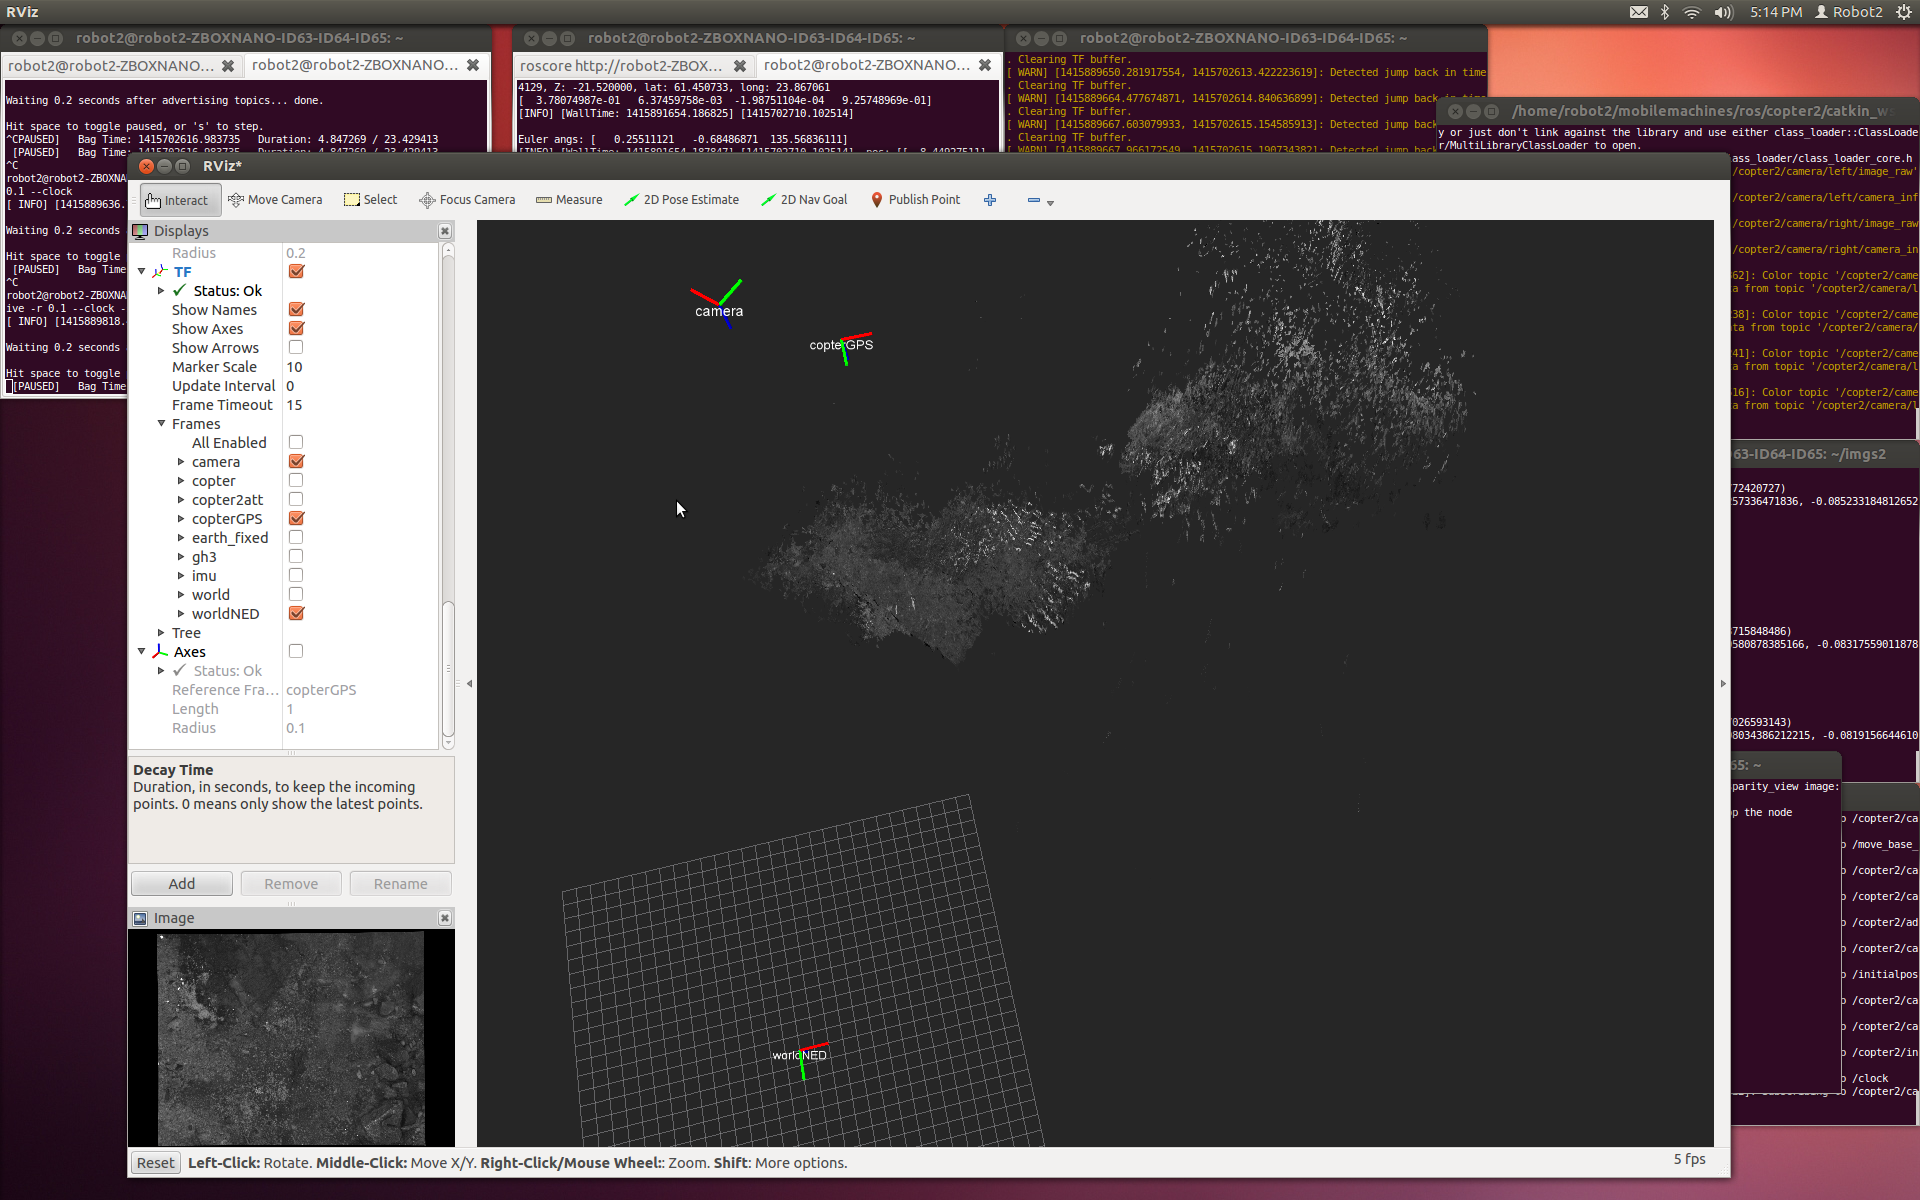
\includegraphics[width=.9\hsize]{screen.png}
\end{frame}

\section{Things to do}
\begin{frame}
\begin{itemize}
  \item Modeling the uncertainties for the SVO
  \item Implementation on ROS
  \item Connecting the filter and SVO (rudimentary work started)
  \item Delay compensation for the GPS measurement
  \item Isolating update steps to smaller submatrices
\end{itemize}

\end{frame}

\section{Work organization}
\begin{frame}
\begin{itemize}
  \item Antti: Making the SVO work on copter data
  \item Tuomas: Making the SVO work on ground vehicle
  \item Joonas: Implementing the scale and orientation estimation
\end{itemize}
\end{frame}


%----------------------------------------------------------------------------------------

\end{document} 